%%%%%%%%%%%%%%%%%%%%%%%%%%%%%%%%%%%%%%%%%%%%%%%%%%%%%%%%%%%%%%%%%%%%%%%%%%%%%%%
%%%%%%%%%%%%%%%%%%%%%%%%%%%%%%%%%%%%%%%%%%%%%%%%%%%%%%%%%%%%%%%%%%%%%%%%%%%%%%%
%%%%%%%%%%%%%%%%%%%%%%%%%%%%%%%%%%%%%%%%%%%%%%%%%%%%%%%%%%%%%%%%%%%%%%%%%%%%%%%
%%%%%%%%%%%%%%%%%%%%%%%%%%%%%%%%%%%%%%%%%%%%%%%%%%%%%%%%%%%%%%%%%%%%%%%%%%%%%%%
\subsection{Describing the Dataset}
\label{sec:dataset}
%%%%%%%%%%%%%%%%%%%%%%%%%%%%%%%%%%%%%%%%%%%%%%%%%%%%%%%%%%%%%%%%%%%%%%%%%%%%%%%
%%%%%%%%%%%%%%%%%%%%%%%%%%%%%%%%%%%%%%%%%%%%%%%%%%%%%%%%%%%%%%%%%%%%%%%%%%%%%%%
%%%%%%%%%%%%%%%%%%%%%%%%%%%%%%%%%%%%%%%%%%%%%%%%%%%%%%%%%%%%%%%%%%%%%%%%%%%%%%%
%%%%%%%%%%%%%%%%%%%%%%%%%%%%%%%%%%%%%%%%%%%%%%%%%%%%%%%%%%%%%%%%%%%%%%%%%%%%%%%

\begin{figure}
    \centering
    \begin{subfigure}[b]{\textwidth}
	\centering
	\includegraphics[width=0.8\textwidth]{Figures/setupCams}
	\caption[Camera setup]{\textbf{Camera setup}}
	\label{fig:cams}
	\vspace{5mm}
    \end{subfigure}
    \begin{subfigure}[b]{\textwidth}
	\centering
	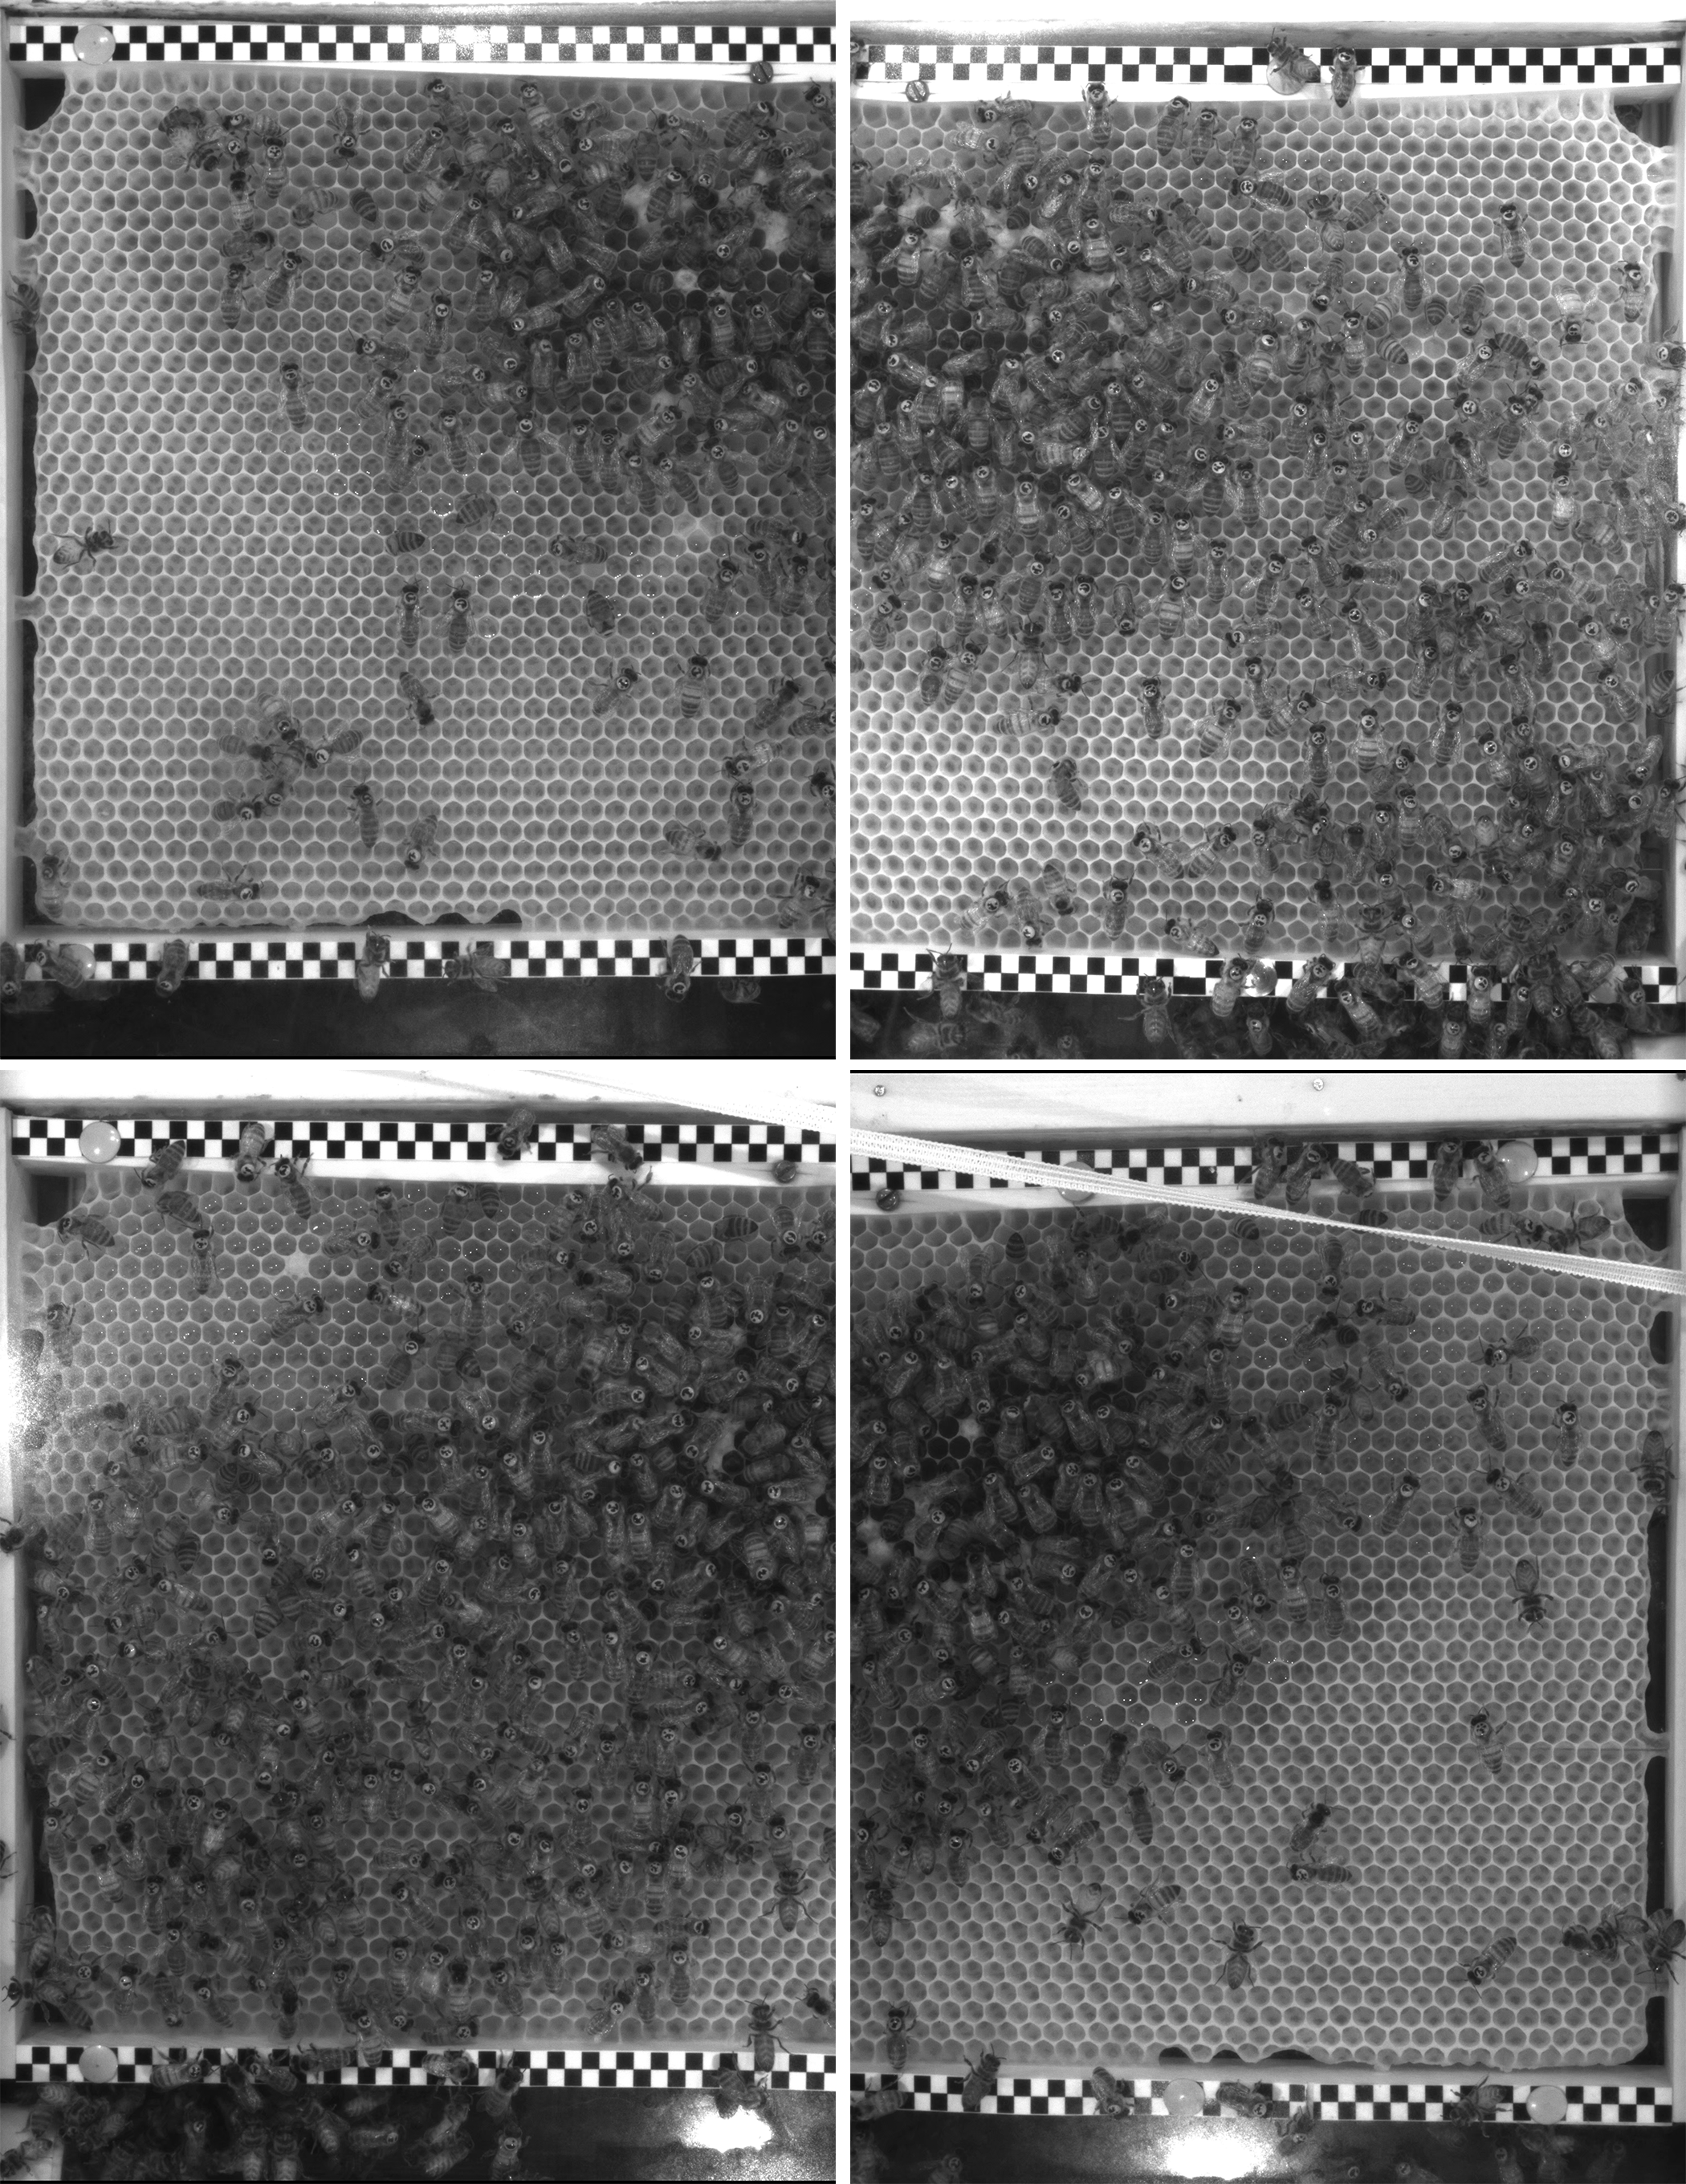
\includegraphics[width=0.65\textwidth]{Figures/beesClose}
	\vspace{5mm}
	\caption[Images for each camera]{\textbf{Images for each camera} Top: side~A, bottom: side~B}
	\label{fig:veryclose}
    \end{subfigure}
 	\caption[Observation setup]{\textbf{Observation setup} Each side of the honeycomb is filmed by two cameras. The two cameras per side overlap, so bees inside this area are detected from both cameras.}
 	\label{fig:obssetup}
\end{figure}

The dataset derives from high-resolution video files that capture tagged honey bees of one colony in a single frame observation hive.
The bees are uniquely tagged with circular 12-bit markers (figure~\ref{fig:markers}, section~\ref{ch:intro}).
Two cameras per side filmed the complete honeycomb permanently.
Figure~\ref{fig:cams} illustrates the camera setup.
The \emph{recording period} lasted nine weeks (63 days), from 19.07.2016 until 19.09.2016, with some interruptions due to maintenance work and technical failures. An overview about the complete recording period is given in figure~\ref{fig:observation-period} in appendix~\ref{ch:appendix}.

All four cameras, each with a resolution of $4000\times3000$ pixels, record $3.5$ frames per second. 
An image analysis pipeline~\cite{wario2015automatic} detects all bees in each frame.
The resulting detection data is stored in a binary file format.
A python library\footnote{The library is called \texttt{bb-binary} and is created by the Biorobotics Lab. It can be found on GitHub: \url{https://github.com/BioroboticsLab/bb_binary}; Last accessed: 2106-02-16, 04:28PM} provides a frame-level access to those binary files.
The size of the dataset is $470$~GB, about $7.5$~GB of binary data per day.

The 67 days long \emph{tagging period} started on 28.06.2016 and lasted until 02.09.2016, resulting in $3.191$ tagged bees. The young bees, which were raised in a separate incubator, were tagged and then added to the observation hive, about noon each day.
Figure~\ref{fig:tagging-period} (Appendix~\ref{ch:appendix}) shows the frequency of tagged bees per day. The hatching day for each bee is documented; therefore the age of each bee at a particular point in time can be calculated.
The life expectancy of a honey bee during summer ranges from 30 to 60 days, according to \textcite[p. 27]{menzel2016intelligenz}
Hence, the maximum number of present bees in the hive is about $1,600$.

For further network analysis, I chose three days: 20., 22., and 24. August.
Those days were chosen because a wide range of age groups was present at this time. The hive especially contained older bees which are likely to be foragers. Besides, no data is missing on those days.

\clearpage
%%%%%%%%%%%%%%%%%%%%%%%%%%%%%%%%%%%%%%%%%%%%%%%%%%%%%%%%%%%%%%%%%%%%%%%%%%%%%%%
%%%%%%%%%%%%%%%%%%%%%%%%%%%%%%%%%%%%%%%%%%%%%%%%%%%%%%%%%%%%%%%%%%%%%%%%%%%%%%%
\subsubsection{Data Scheme}
\label{subsec:datascheme}
%%%%%%%%%%%%%%%%%%%%%%%%%%%%%%%%%%%%%%%%%%%%%%%%%%%%%%%%%%%%%%%%%%%%%%%%%%%%%%%
%%%%%%%%%%%%%%%%%%%%%%%%%%%%%%%%%%%%%%%%%%%%%%%%%%%%%%%%%%%%%%%%%%%%%%%%%%%%%%%

\begin{table}[!t]
\colorbox{usethiscolorhere}{
\centering
\begin{tabularx}{\textwidth}{@{} r Y @{}}
	\textbf{Frame container} &
	Contains all frames, which belong to a specific video file of a certain camera.\\
	\textbf{Frame} &
	Includes all detections of one frame at a certain point in time.\\
	\textbf{Detection} &
	Detection of a bee at a certain point in time.\\
	\textbf{Decoded ID} &
	Identifier of a bee consisting of 12 probability values, representing 12 bits.\\
	\textbf{Confidence} &
	Value between 0\% and 100\%.\\
	\textbf{ID} &
	Decimal representation of a decoded ID.\\
	\textbf{Bee time series} & Binary sequence, indicating the absence and presence of a certain bee in a particular time interval.\\
	\textbf{Pair time series} & Binary sequence, indicating whether or not two bees are close to each other, in a particular time interval.\\
\end{tabularx}
}
\end{table}

The data is organized in so-called \emph{frame containers}.
Each frame container corresponds to one video file of a certain camera and consists of about $1024$ frames.
Each \emph{frame} holds a list of bees, which were detected by the image analysis pipeline.

A bee \emph{detection} has, among others, the following attributes:

\begin{table}[!h]
\centering
\begin{tabular}{rl}
\textbf{xpos}: & $x$ coordinate of bee with respect to the image in pixel \\
\textbf{ypos}: & $y$ coordinate of bee with respect to the image in pixel \\
\textbf{decoded ID}: & decoded 12-bit ID \\
\textbf{cam ID}: & ID of the camera ${0,1,2,3}$ \\
\textbf{timestamp}: & unix timestamp with milliseconds\\
\end{tabular}
\end{table}

The data can be accessed by iterating on the frame level, using a start and end time\-stamp for specifying a time interval. The complete data scheme can be found on GitHub\footnote{\url{https://github.com/BioroboticsLab/bb_binary/blob/master/bb_binary/bb_binary_schema.capnp}; Last accessed: 2106-02-16, 04:46PM}. 


%%%%%%%%%%%%%%%%%%%%%%%%%%%%%%%%%%%%%%%%%%%%%%%%%%%%%%%%%%%%%%%%%%%%%%%%%%%%%%%
%%%%%%%%%%%%%%%%%%%%%%%%%%%%%%%%%%%%%%%%%%%%%%%%%%%%%%%%%%%%%%%%%%%%%%%%%%%%%%%
\subsubsection{ID Probabilities, Confidence Level, and Quality}
\label{subsec:confidence}
%%%%%%%%%%%%%%%%%%%%%%%%%%%%%%%%%%%%%%%%%%%%%%%%%%%%%%%%%%%%%%%%%%%%%%%%%%%%%%%
%%%%%%%%%%%%%%%%%%%%%%%%%%%%%%%%%%%%%%%%%%%%%%%%%%%%%%%%%%%%%%%%%%%%%%%%%%%%%%%

\begin{figure}
    \centering
    \begin{subfigure}[b]{0.45\textwidth}
        \includegraphics[width=\textwidth]{Figures/detectionsWrongConf}
        \caption[Detections]{\textbf{Detections}}
        \label{fig:detections}
    \end{subfigure}
    \begin{subfigure}[b]{0.45\textwidth}
        \includegraphics[width=\textwidth]{Figures/idsWrongConf}
        \caption[IDs]{\textbf{IDs}}
        \label{fig:ids}
    \end{subfigure}
 	\caption[Quality of detections and IDs]{\textbf{Quality of detections and IDs} \emph{Light green} represents the number of remaining detections and IDs (from $4096$ possible IDs). \emph{Dark green} indicates the fraction of invalid detections and IDs and in relation to the remaining number of detections and IDs.\protect\footnotemark}
 	\label{fig:remainingVSquality}
\end{figure}

\footnotetext{Data set: 26.07.2016, 4~p.~m., 10~minutes, all cameras}

Twelve bits can encode the identity of 4096 bees.
Each bit of the decoded ID is not a one or zero but represents a probability between $0$ and $255$, normalized to a value between $0$ and $1$.
Therefore, a bit indicates the confidence of the image analysis pipeline for that specific bit.
I define the confidence $c$ for a bit $b$, analogously to Leon~\textcite[p.~14]{leon2016}, as $c(b)=2\cdot|b-0.5|$.
The confidence of a decoded ID is, accordingly, the minimum of all twelve bits' confidences.
Detections with a confidence below a certain level are removed from the data set.
Consequently, a high level of confidence reduces the amount of data, which remains for further processing.

I use the age information of the bees to check the quality of the remaining data.
A bee has a negative age, if the pipeline detected a code, that was not used yet.
I examined the number of remaining bee detections and IDs, depending on the chosen confidence by calculating the age of each bee detection and ID.
A bee detection with a negative age is counted as an \emph{invalid detection}. Also, an ID with a negative age is counted as an \emph{invalid ID}.

As expected, with increasing confidence, the number of remaining detections and IDs decreases (figure~\ref{fig:remainingVSquality}), as well as the fraction of invalid detections and IDs.
With a confidence level of 100\%, the fraction of invalid detections reaches the value of 2.5\%. However, the fraction of invalid IDs stays at the high value of 30.2\%. Consequently, selecting a high level of confidence is not sufficient for obtaining a high data quality.
Therefore, to obtain a more reliable dataset, invalid detections need to be filtered out, in addition to choosing a good level of confidence.

%%%%%%%%%%%%%%%%%%%%%%%%%%%%%%%%%%%%%%%%%%%%%%%%%%%%%%%%%%%%%%%%%%%%%%%%%%%%%%%
%%%%%%%%%%%%%%%%%%%%%%%%%%%%%%%%%%%%%%%%%%%%%%%%%%%%%%%%%%%%%%%%%%%%%%%%%%%%%%%
\subsubsection{Time Series of Bees and Bee Pairs}
\label{subsec:tracking}
%%%%%%%%%%%%%%%%%%%%%%%%%%%%%%%%%%%%%%%%%%%%%%%%%%%%%%%%%%%%%%%%%%%%%%%%%%%%%%%
%%%%%%%%%%%%%%%%%%%%%%%%%%%%%%%%%%%%%%%%%%%%%%%%%%%%%%%%%%%%%%%%%%%%%%%%%%%%%%%

The dataset is transformed into binary \emph{bee time series}, depicted in figure~\ref{fig:structure} (left and middle). A time series of a bee is a sequence of zeros and ones indicating the absence and presence of a bee over a specified time interval.
I examined the effect the level of confidence has on the bee time series.
As expected, with an increasing confidence level the average gap length decreases and the overall number of gaps increases (figure~\ref{fig:gaps}).

The number of gaps, those bee time series has, is important because in a later step I want to extract pairs of close bees, who are present at the very same time. I call those \emph{pair time series}, as shown in figure~\ref{fig:structure} (right). So a lot of gaps in bee time series could lead to a lot of gaps in the pair time series.

\begin{figure}[htb]
	\centering
	\includegraphics[width=1.0\textwidth]{Figures/structure}
	\caption[Structure of dataset]{\textbf{Structure of dataset} \emph{Left}: original dataset - containing a sequence of frames with bee detections; \emph{Middle:} binary bee time series - zero and one indicate absence and presence of a bee; \emph{Right:} binary pairs time series - zero and one indicate the absence and presence of two bees in the same frame.}
	\label{fig:structure}
\end{figure}

\begin{figure}[htb]
	\centering
	\begin{subfigure}[b]{0.45\textwidth}
		\includegraphics[width=\textwidth]{Figures/gaplen}
		\caption[Length of gaps]{\textbf{Length of gaps}}
		\label{fig:gaplen}
	\end{subfigure}
	\begin{subfigure}[b]{0.45\textwidth}
		\includegraphics[width=\textwidth]{Figures/numgaps}
		\caption[Number of gaps]{\textbf{Number of gaps}}
		\label{fig:numgaps}
	\end{subfigure}
	\caption[Influence of Confidence Level on Gaps]{\textbf{Influence of confidence level on gaps} [TODO: add legend][TODO:gaps D] With an increasing level of confidence the average gap length decreases and the number of gaps per bee series increases. \emph{Orange} indicates the median, \emph{green the mean}.\protect\footnotemark }
	\label{fig:gaps}
\end{figure}

\footnotetext{Data set: 26.07.2016, 16:00-16:05}


%%%%%%%%%%%%%%%%%%%%%%%%%%%%%%%%%%%%%%%%%%%%%%%%%%%%%%%%%%%%%%%%%%%%%%%%%%%%%%%
%%%%%%%%%%%%%%%%%%%%%%%%%%%%%%%%%%%%%%%%%%%%%%%%%%%%%%%%%%%%%%%%%%%%%%%%%%%%%%%
\subsubsection{Detection Frequency Filter}
%%%%%%%%%%%%%%%%%%%%%%%%%%%%%%%%%%%%%%%%%%%%%%%%%%%%%%%%%%%%%%%%%%%%%%%%%%%%%%%
%%%%%%%%%%%%%%%%%%%%%%%%%%%%%%%%%%%%%%%%%%%%%%%%%%%%%%%%%%%%%%%%%%%%%%%%%%%%%%%
A good indicator, whether a bee is alive and present on a particular day, is its detection frequency. The hypothesis is: Bees who have a low detection rate are not physically present in the hive, respectively do not exists at that day.
To check this hypothesis, I investigate whether there is a correlation between the age of bees and their detection frequency.

\begin{figure}[t]
	\centering
	\includegraphics[width=1.0\textwidth]{Figures/filter}
	\caption[Detection frequency of IDs]{\textbf{Detection frequency of IDs} [TODO: add legend] \emph{Orange} coressponds to bees with a negative age and \emph{green} displays bees with a positive age.\protect\footnotemark}
	\label{fig:filter}
\end{figure}

\footnotetext{Data set: 20.08.2016, 24 hours, number of total frames: 302400}

Bess with a negative age are on average detected less frequently than bees with a positive age.
In advance, I excluded bees from the statistics, which had a negative age, but a detection frequency over 10000 frames. Their detection frequency is similar to that from bees with a positive age. I looked at the corresponding photos taken by the camera and confirmed that those are living bees and no artifacts.\footnote{Probably a mistake in the table, which reports the hatching days for each bee.}
Also I excluded bees~($n=10$), whose age is unknown\footnote{id= [2,
    74,
    2045,
    3172,
    3764,
    3796,
    3827,
    3836,
    3844,
    3940]}.

For each analysis day, the number of detections per ID is obtained, excluding the mentioned IDs.
Additionally, I discarded all detections with an ID frequency below the 99th percentile of negative IDs.
A list of valid IDs per day is kept to filter out wrong detections beforehand.

%%%%%%%%%%%%%%%%%%%%%%%%%%%%%%%%%%%%%%%%%%%%%%%%%%%%%%%%%%%%%%%%%%%%%%%%%%%%%%%
%%%%%%%%%%%%%%%%%%%%%%%%%%%%%%%%%%%%%%%%%%%%%%%%%%%%%%%%%%%%%%%%%%%%%%%%%%%%%%%
\subsubsection{Implications}
%%%%%%%%%%%%%%%%%%%%%%%%%%%%%%%%%%%%%%%%%%%%%%%%%%%%%%%%%%%%%%%%%%%%%%%%%%%%%%%
%%%%%%%%%%%%%%%%%%%%%%%%%%%%%%%%%%%%%%%%%%%%%%%%%%%%%%%%%%%%%%%%%%%%%%%%%%%%%%%
[TODO: redo]\\
The confidence level is set to 95\%.
This a good balance between gaps in the time series and quality of the data and amount of remaining data.
Because bee time series contain a lot of short gaps (mean = 3, 95\% confidence), the inference of edges (bees that are spatially close to each other at the same time), should take this into account.